%% TODO fix the case study so that the time complexity is not as high
%% TODO say what operator will be used, why it's good and what the alternatives are
%% TODO say what the issues with rank-based selection are and why it's a good fit here
%% TODO say what the issues with cross-over are and why / why not it's a good fit here
%% TODO is the phenotype the timetable OR a list of lectures?

%% options: [no]titlepage, twocolumn, landscape, draft
\documentclass[a4paper, 12pt, titlepage]{article}
\usepackage{graphicx}
\usepackage{titlesec}

\titlespacing*{\section}
{0pt}{1.0ex plus 1ex minus .2ex}{1.0ex plus .2ex}
\titlespacing*{\subsection}
{0pt}{1.0ex plus 1ex minus .2ex}{1.0ex plus .2ex}
\usepackage[utf8]{inputenc}
\usepackage[english]{babel}
\usepackage[margin=0.1in]{geometry}

\usepackage{minted}
\date{} % overwrite default format
\author{Norbert Logiewa\\nl253}
\title{Applications of Evolutionary Algorithms in \\Scheduling, Planning and Timetabling}

\begin{document}

\maketitle

Evolutionary algorithms (EA) are a class of procedures that are used when
finding a solution to a problem using regular means is not possible
or very difficult.  This essay will discuss how GA can be applied
to scheduling.  \emph{Scheduling} and \emph{timetabling} in this essay
will refer to ordering of tasks that aims to maximise the productivity.
The ordering may schedule some activities to take place in parallel if
business rules and the amount of resources allow for that.  Efficient
scheduling of tasks if of interests to anyone who wishes to increase their
productivity \emph{without} investing additional resources.  EAs allow
to find good-enough solution to problems that don't necessarily need an
\emph{optimal} solution\cite[p.~44]{heaton2014}.  This is often because
the search space is too large to be directly traversed so brute-force
methods are not possible.

% \emph{Productivity} will refer the extent to which a schedule helps some
% organisation to achieve their goals. \footnote{If, for example, we are
% scheduling for a web development agency, we can measure productivity by
% the lines of code produced by the developers.}

\section*{Case Study -- University}

A hypothetical university may wish to improve the productivity of students
and lecturers by using an EA for timetabling. Suppose the university
offers 200 modules to 16000 students. Each year every student must take 8
unique modules. Each module needs to have 2 one-hour lectures during the
working week. Additionally, each of those lectures or can take place in
one of 50 lecture halls. Moreover, each of those lectures may be given
by a lecturer from the relevant department.  Finally, each lecture or
may take place a time between 9am and 7pm.  The task would be to ensure
that: every student and lecturer is in at most one lecture at a time,
only one lecture takes place in a lecture hall at the same time, etc.
A timetable i.e. a candidate solution that obeys all of these business
rules would be favoured in the process of natural selection and would
receive a higher fitness score as evaluated by the fitness function.

% As input the GA would take a set of combinations of modules that the students chose.

\section*{Solving the Problem}

GA is well suited for the task because there is likely many good-enough
solutions to the problem i.e. many timetables could satisfy the
constraints listed above. In other words, the fitness landscape has
many peaks, hence, using a global-search algorithm is beneficial.
Furthermore, the complexity of the problem (large search
space and multiple dimensions) means that a brute force search in this
multi-dimensional space would take too much time.

\subsection*{Phenotype and Genotype}

Each candidate solution (timetable) would be encoded as a bit-string
\footnote{this is the genotype and is analogous to DNA} representing all
the lectures along with time, place and the lecturer taking place during
the week.  This choice of encoding i.e. genotype is because bit-string
encoding has been the most studied in the literature on GA and as a
result the operators invented by researchers assume this encoding for
each candidate. \cite[p.~103]{eberhart2007}. The crossover operator,
for instance, is extremely easy to apply to a bit-string but less easy
to other data structures such as sets. We might allocate a chunk of bits
for every lecture that must take place.  In every sub-string representing
a lecture the first bit would determine whether the lecture takes place
in the first or the second semester.  The following \(m\) bits could
encode an integer index in the modules array.  The next \(l\) bits could
encode an integer index in our lecturer array. The following \(t\) bits
could encode an integer referring to the time that lecture will take
place. The last \(h\) bits could encode an integer index in our lecture
halls array. Hence each lecture would be a bit-string of length \(1 +
m + l + t + h\) and each candidate would be a concatenation of \(400\)
of these giving us in total a bit-string of length \(400(1 + m + l + t +
h)\). If we delegate, say, 16 bits to representing the time and 8 for each
indexing integer, we end up with each candidate having a size of \(400 *
(1 + 8 + 8 + 8 + 16) bits = 16400 bits = 2050 Bytes = approx. 2KB \).
The \emph{phenotype} might be a list of lectures, for instance, which
we would decode from the genotype (bitstring).

\subsection*{Selection Operator}

A good choice of selection operator would be rank-based selection. The
reason for this is that in this scenario the exact fitness value of
an individual is irrelevant. Another reason is that it simplifies
implementation. An alternative would be using roulette selection.

\subsection*{Genetic Operators \& Adaptive GA}

Since as a result of this selection the population size has depleted
pairs of winners are used as input to the crossover operator to
create new individuals.  Crossover is used because it is a standard
and well-understood operator.  Additionally, mutation with a small
probability would be introduced to further increase variation in the
population. A good starting values for the parameters would be as follows:
\(p(crossover) = 0.8\) and \(p(mutation) = 0.2\) \cite{heaton2014}.

However, the crossover operator is problematic. In the initial phase of
looking for a solution across the fitness landscape it is useful to vary
candidates a lot so using crossover is highly beneficial. However, once
a satisfactory candidate has been found, we might only wish to tweak it
a bit. Altering the candidate too much would be equivalent to abandoning
the progress that has been made to reach this fitness score. Hence,
a less "invasive" and more fine-grained operator such as mutation may
become more advantageous as the number of iterations grows. We could use
it to target smaller parts of the bitstring. In essence, the benefit of
using crossover, arguably, diminishes with time. To implement that we
might make the probability of mutation and cross-over be a function of
the number of iteration. \(p(mutation)\) might grow proportionally to
time until it reaches \(1.0\) and \(p(cross-over)\) might become smaller
proportionally to time until it reaches \(0.0\). This is referred to as 
an \emph{adaptive} GA.

An alternative way of preserving the fittest candidates in the next
population would be to use elitism. This would protect against degrading
of solutions when cross-over is applied to fittest candidates.

\subsection*{The fitness function}

The fitness function would decipher each of the \(400\) sub-strings within each
candidate bit-string and assign a score to each candidate which would reflect
the extent to which it obeys the business rules. In pseudo (python-like) code: 

\inputminted{python}{fitness.py}

The pseudocode illustrates that the fitness function has a bad \(O(l^2 *
c)\) complexity where: \(l\) = number of lectures \footnote{in this
scenario \(l = 200 * 2\)} for all modules and \( c = \) number of
combinations of modules.  Initially it may seem that the fitness function
is not computationally feasible.  With 200 modules and 8 modules to be
takes for every student the maximum number of combinations is \(8C200 =
55098996177225\). However, there are bound to be restrictions on the
combinations of modules. For example, a computer science student is
unlikely to be allowed to take "Introduction to Criminology". In fact, we
would expect each student to only be able to choose from around 15 modules
from their own department. \(8C15 = 6435\) is a much more manageable number.
\footnote{the pseudo-code assumes that module configurations for all students are presented
in a multiset where every key is itself a set of modules (similar to frozen sets in
Python, see https://docs.python.org/3/library/stdtypes.html#frozenset)
and value is the number of students who chose this particular combination of modules}

\subsection*{The invariant}

The procedure would be repeated until either 10 minutes have passed or a
solution with a satisfactory fitness score has been found.  At that point
the best timetable (fittest individual) in our population is presented
as the solution to the timetabling problem.

% The idea is that the quality of the solution \emph{increases} the longer
% the algorithm is being run. \footnote{EAs are \emph{greedy algorithms}.}

\section*{Summary}

The basic idea behind this particular version of GA is described by the
following UML activity diagram: 

\begin{figure}[h]
    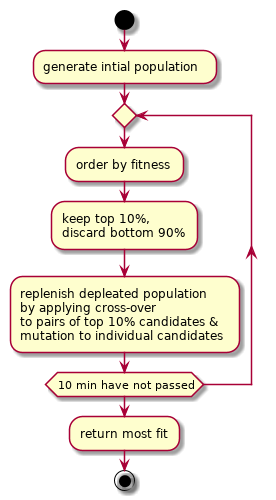
\includegraphics[scale=0.6]{algo.png}
    \centering
\end{figure}

This essay demonstrated how EA can be used to aid timetabling and
scheduling. It illustrated how to apply EA using a case study of a
university, it discussed how to encode the candidate timetables and
stated how carry out the algorithm in this scenario.

\begin{thebibliography}{9}

  %% 1 authors
  %% 2 title of the paper
  %% 3 name of conference/journal/book where it was published
  %% 4 number of the volume and issue in the case of journals
  %% 5 page numbers of the paper
  %% 6 publisher
  %% 7 year or month and year for journals
  
  \bibitem{norvig2010}
  Stuart Russel and Peter Norvig,
  \textit{Artificial Intelligence},
  \textit{A MODERN APPROACH},
  p. 126-129, 
  p. 155,
  3rd Ed., 
  Pearson Education
  2010.

  \bibitem{floreano2008}
  Dario Floreano and Claudio Mattiussi,
  \textit{Bio-Inspired Artificial Intelligence},
  \textit{THEORIES, METHODS, AND TECHNOLOGIES},
  p. 1-38,
  MIT Press,
  2008.

  \bibitem{eberhart2007}
  Russel C. Eberhart,
  \textit{Computational Intelligence},
  \textit{Concepts to Implementations},
  p. 103-118,
  p. 51-68,
  Denise E.M. Penrose,
  2007.

  \bibitem{heaton2014}
  Jeff Heaton,
  \textit{Artificial Intelligence for Humans},
  \textit{Volume 2: Nature Inspired Algorithms},
  p. 1-100,
  Heaton Research, Inc,
  2014.

\end{thebibliography}

\end{document}
